\documentclass{article}
\usepackage{graphicx}
\usepackage{subcaption}
\usepackage{amsmath}
\usepackage{cite}  % Optional for better citation management
\usepackage{placeins}

\title{Weekly meeting notes}
\author{Eugenio Pescimoro }

\begin{document}

\maketitle

\section{Introduction}
The aim of these notes is to describe the numerical modelling of solute transport and diffusion through fractured porous media using a random walk approach.

\FloatBarrier  % Prevents figures from floating past this point
\section{Diffusion in fractures}
The drifting term..

\FloatBarrier  % Prevents figures from floating past this point
\section{Code verification}
As a first step for ensuring the reliability of a solute transport simulation code it is essential to verify that the solutions of numerical experiments and analytical study coincide. For this purpose we compare the analytical solutions from three different transport problems against the numerically generated results, namely:
\begin{itemize}
    \item spatial distribution of the concentration at a given time for a solute that is displaced through an infinite bi-dimensional domain with horizontal impenetrable boundaries and initial one-dimensional vertical location;
    \item probability density function of a breakthrough curve for a solute which is displaced through a semi-infinite domain where particles' arriving times are recorded on a vertical absorbing control plane;
    \item the survived particle in time curve for a solute subject to an exponential degradation process. 
\end{itemize}

\subsection{Infinite domain}
In this test (Figure \ref{fig:Infinite}) we release $10^4$ particles in a horizontally infinite domain. Reflecting properties are assigned to the upper and lower horizontal boundaries and the simulation is run for $10^3$ time steps. After $10^2$ time steps the spatial distribution of the solute is recorded and compared against the analytical solution at the same time, namely:
\begin{equation}
    c(x) = \frac{e^{-\frac{x^2}{4 D t}}}{\sqrt{4 \pi D t}}.
\end{equation}

\begin{figure}[htbp]
    \centering
    \begin{subfigure}[b]{0.3\textwidth}
        \centering
        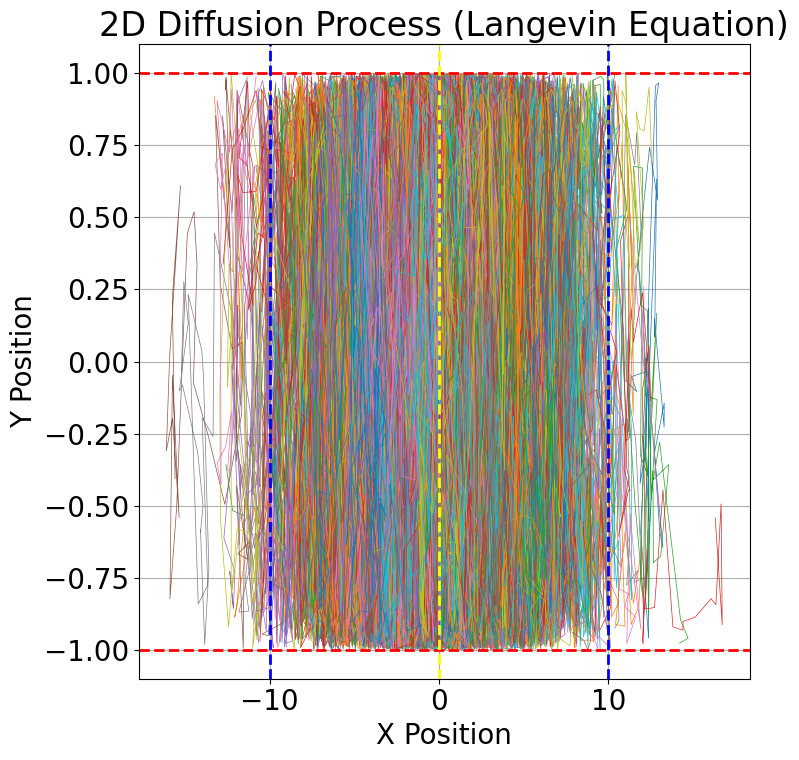
\includegraphics[width=\textwidth]{images/trajectoriesInfinite.png} % Replace with your image path
        \caption{Trajectories of 1e4 particles during 1e3 time steps}
        \label{fig:subplotTrInf}
    \end{subfigure}
    \hfill
    \begin{subfigure}[b]{0.3\textwidth}
        \centering
        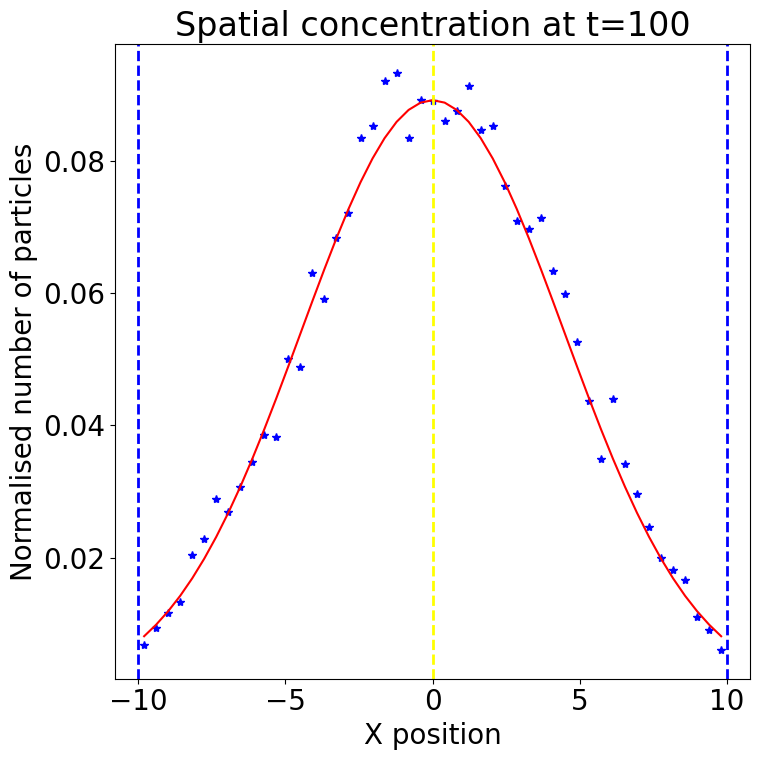
\includegraphics[width=\textwidth]{images/verificationInfinite1e4.png} % Replace with your image path
        \caption{Spatial distribution of the particles at time 1e2}
        \label{fig:subplotVerInf}
    \end{subfigure}
    \hfill
    \begin{subfigure}[b]{0.3\textwidth}
        \centering
        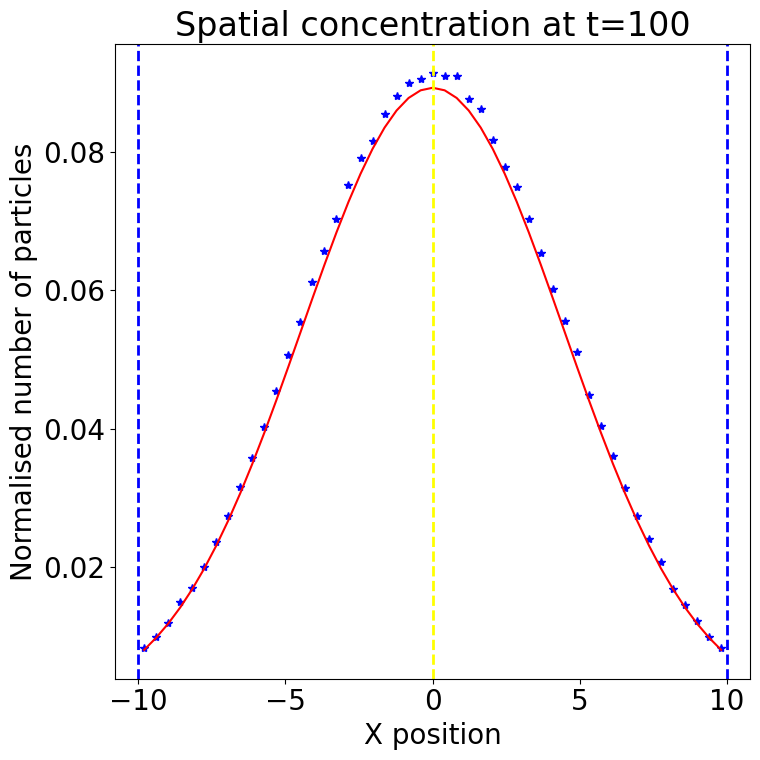
\includegraphics[width=\textwidth]{images/verificationInfinite1e6.png} % Replace with your image path
        \caption{Spatial distribution of the particles at time 1e2 with 1e5 particles}
        \label{fig:subplotVerInf1e5}
    \end{subfigure}
    \caption{Verification of the code comparing two spatial distribution of the concentration at a given time: solid blue line represents the spatial concentration from a numerical simulation while solid red line shows the analytical solution of the spatial concentration in a infinite domain at the same given time.}
    \label{fig:Infinite}
\end{figure}

\subsection{Semi-infinite domain}
In this test (Figure \ref{fig:SemiInfinite}), the arrival times of the particles are recorded on the left absorbing boundary. The spatial bins are logarithmically spaced and the number of particles per time bin is divided by the total number of particles and the width of the temporal bin. This result is compared against its analytical solution, namely:
\begin{equation}
        c(t) = \frac{x_0 e^{-\frac{x_0^2}{4 D t}}}{\sqrt{4 \pi D t^3}}
\end{equation}
where $x_0$ is the distance between the vertical plane where particle are released and the absorbing vertical plane.

\begin{figure}[htbp]
    \centering
    \begin{subfigure}[b]{0.3\textwidth}
        \centering
        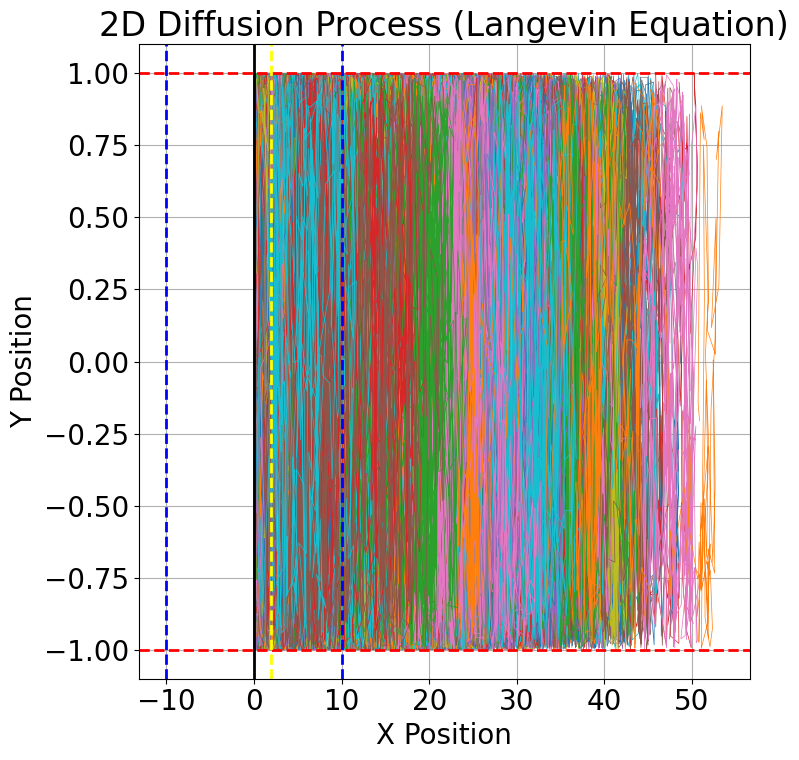
\includegraphics[width=\textwidth]{images/trajectoriesSemiInfinite.png} % Replace with your image path
        \caption{Trajectories of 1e4 particles during 1e3 time steps}
        \label{fig:subplotTrSemiInf}
    \end{subfigure}
    \hfill
    \begin{subfigure}[b]{0.3\textwidth}
        \centering
        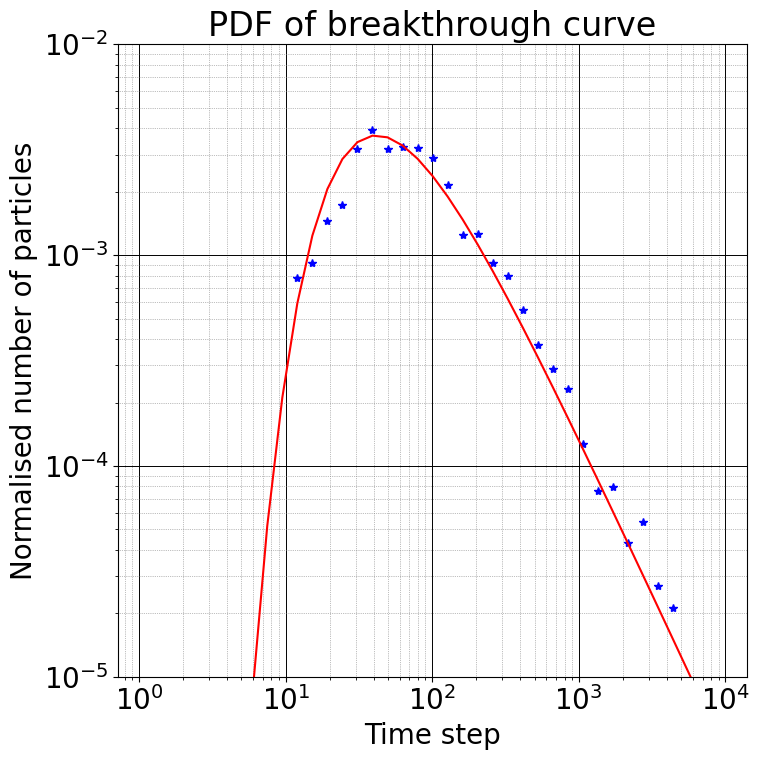
\includegraphics[width=\textwidth]{images/verificationSemi-infinite1e3.png} % Replace with your image path
        \caption{Arrival times on the left absorbing boundary}
        \label{fig:subplotVerSemiInf}
    \end{subfigure}
    \hfill
    \begin{subfigure}[b]{0.3\textwidth}
        \centering
        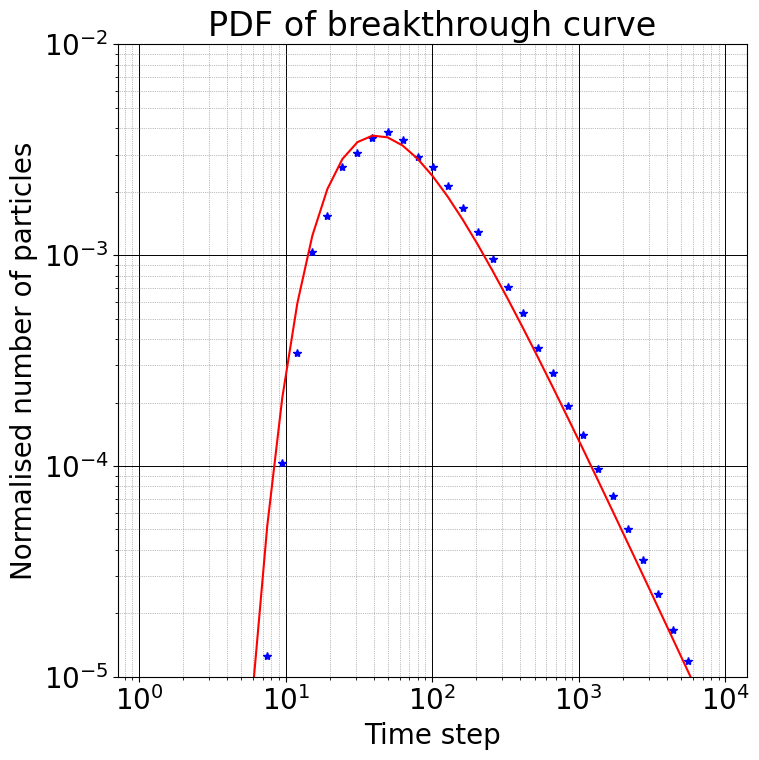
\includegraphics[width=\textwidth]{images/verificationSemi-infinite1e5.png} % Replace with your image path
        \caption{Arrival times on the left absorbing boundary with 1e4 particles, 1e4 time steps and x0=4}
        \label{fig:subplotVerSemiInfImproved}
    \end{subfigure}
    \caption{Verification of the code comparing two pdfs of the btc: blue dots represent the btc pdf from numerical simulation, solid red line is the analytical solution of the btc pdf for a semi-infinite domain}
    \label{fig:SemiInfinite}
\end{figure}

\subsection{Degradation}
This test (Figure \ref{fig:Degradation}) focuses on a horizontally infinite scenario where $10^3$ particles travel for maximum $10^3$ time steps. The upper and lower horizontal boundaries are both reflecting the particles however, some of the latter disappear due to a degradation process which follows an exponential trend:
\begin{equation}
    p_s(t) = k e^{-kt}
\end{equation}
where $p_s(t)$ is the survival probability distribution. Before the simulation, the survival probability of each particle is a random variable charaterised by the $p_s(t)$ probability distribution with values between 0 and the maximum number of time steps. After every time step, the particles' survival time is withdrawn from the simulation if its survival time is less than the time step. The degradation kinetic constant $k$ for the following simulation was assigned an arbitrary value equal to 0.01.

\begin{figure}[htbp]
    \centering
    \begin{subfigure}[b]{0.45\textwidth}
        \centering
        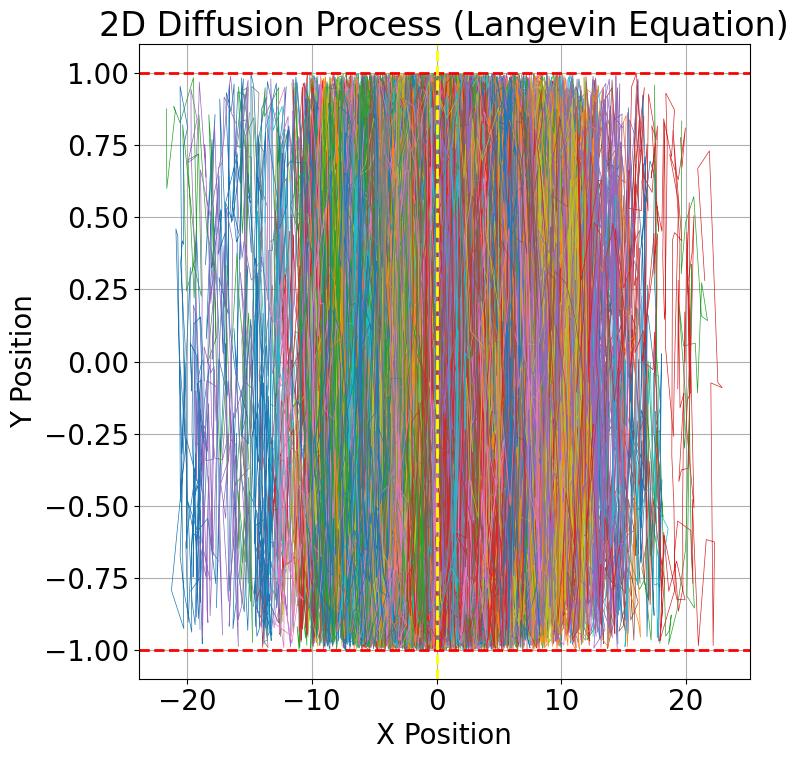
\includegraphics[width=\textwidth]{images/trajectoriesDegradation.png} % Replace with your image path
        \caption{Trajectories of 1e3 particles during 1e3 time steps with degradation}
        \label{fig:subplotTrDeg}
    \end{subfigure}
    \hfill
    \begin{subfigure}[b]{0.45\textwidth}
        \centering
        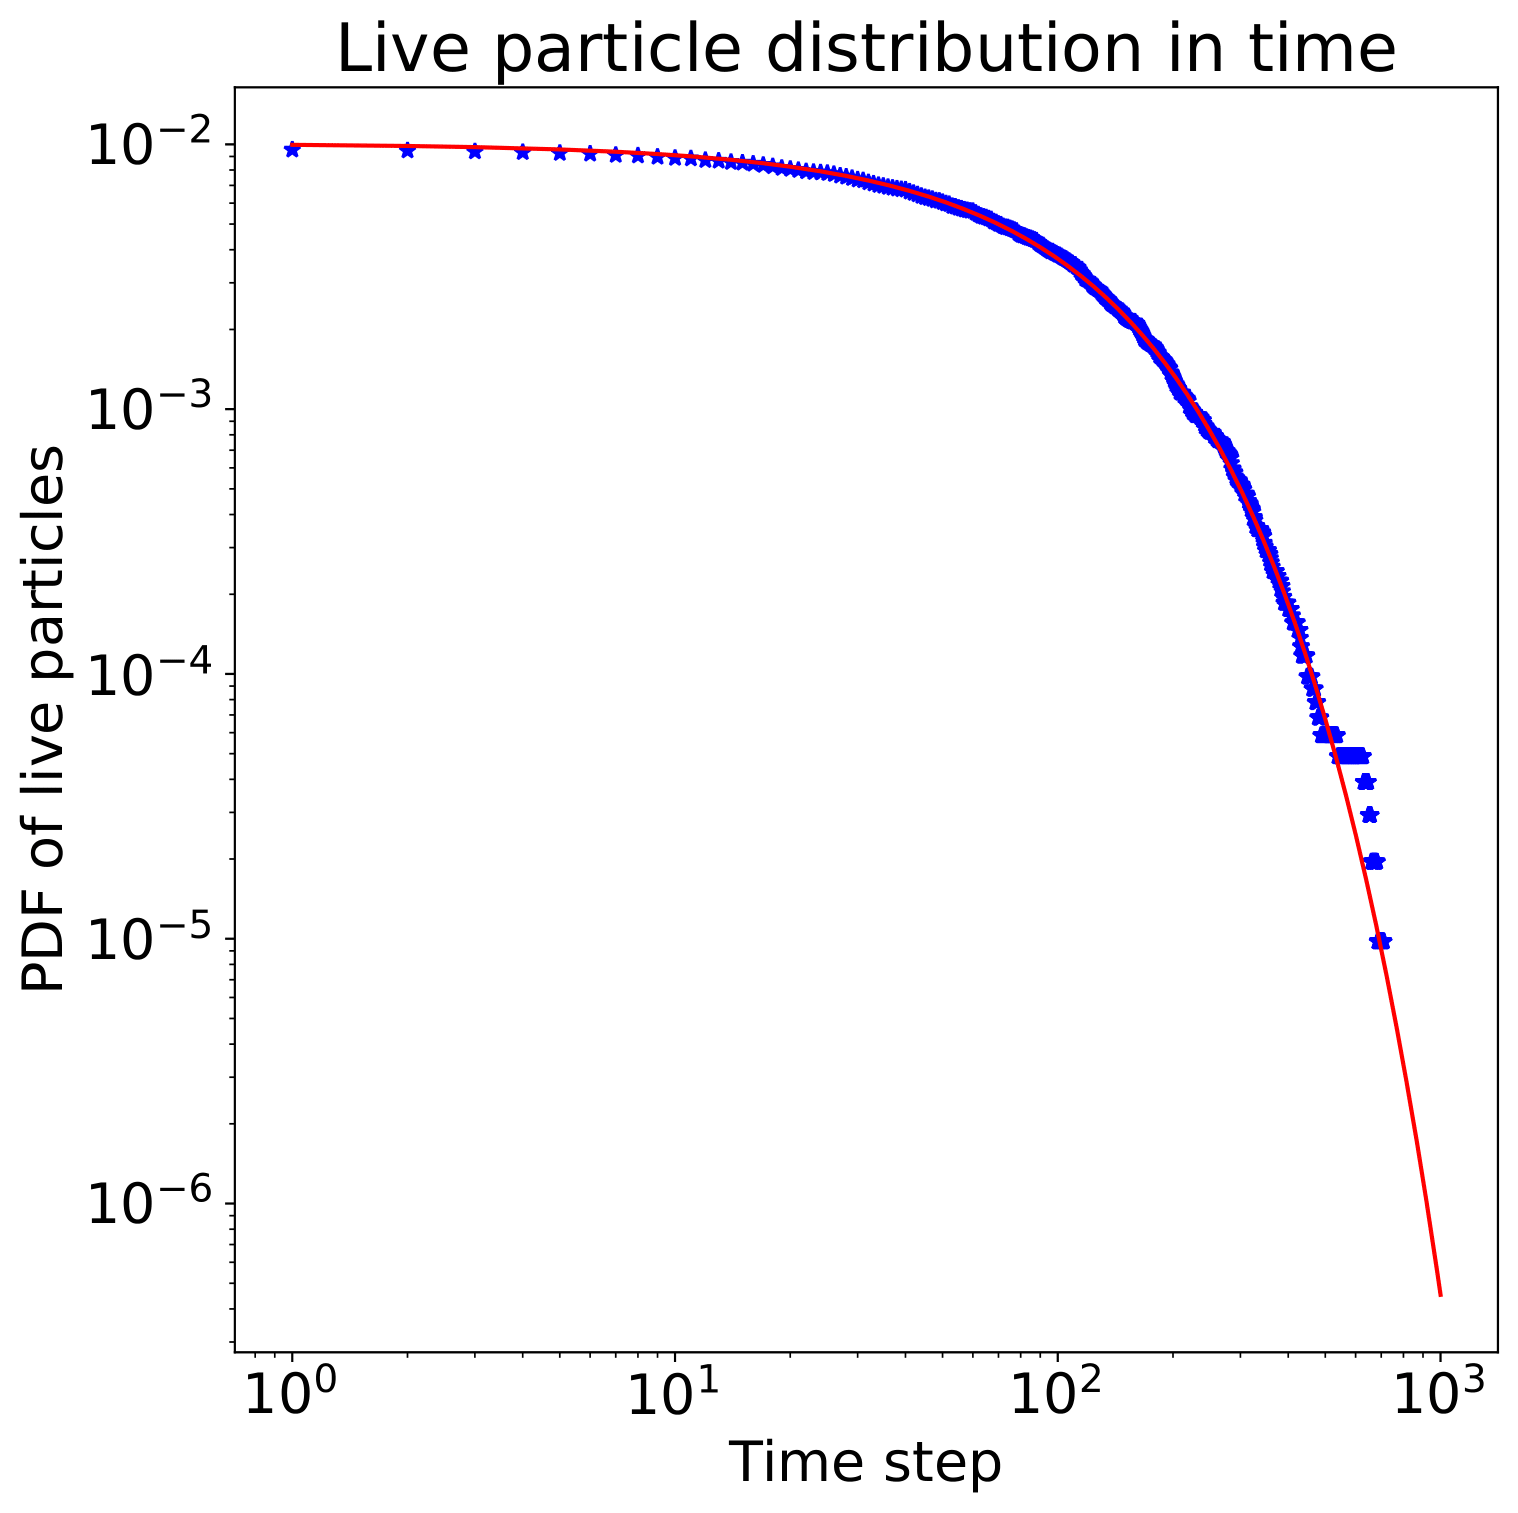
\includegraphics[width=\textwidth]{images/liveParticleInTime.png} % Replace with your image path
        \caption{PDF of survived particles in time}
        \label{fig:subplotLivePart}
    \end{subfigure}
    \caption{Verification of the code comparing two pdfs of the btc: blue dots represent the btc pdf from numerical simulation, solid red line is the analytical solution of the btc pdf}
    \label{fig:Degradation}
\end{figure}

\FloatBarrier  % Prevents figures from floating past this point
\section{Absorbing boundaries}
For the case where the particles which impact the lower and upper boundaries are absorbed, the analytical solution is not available. In the following example (Figure \ref{fig:finalPos} - Figure \ref{fig:AbsorptionInTime}), the particles which hit the boundaries have 100\% probability of being absorbed. An alternative which has been implemented in the code but is not currently shown allows to assign to the particles different absorption probability that is, the outcome of the impact of particle with the walls (either reflected or absorbed) will becomes a random variable which is drawn from a custom probability distribution.

\subsection{Final positions}
The final position of $10^4$ particles after 20 steps is shown in Figure \ref{fig:finalPos}.
\begin{figure}[h]
    \centering
    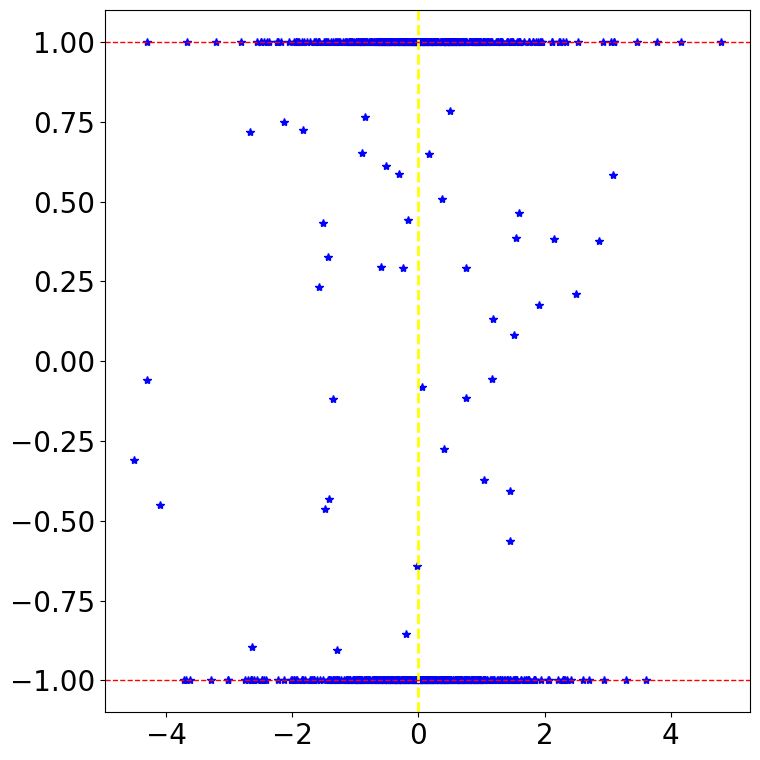
\includegraphics[width=0.5\textwidth]{images/finalPositions.png}
    \caption{Final position for 1e4 particles after 20 steps in a domain characterised by absorbing boundaries}
    \label{fig:finalPos}
\end{figure}

\subsection{Cross section histograms}
Figures \ref{fig:subplotVertFinal} and \ref{fig:subplotHorFinal} show the number of particles in two different regions of space at the end of the simulation. 
\begin{figure}[htbp]
    \centering
    \begin{subfigure}[b]{0.45\textwidth}
        \centering
        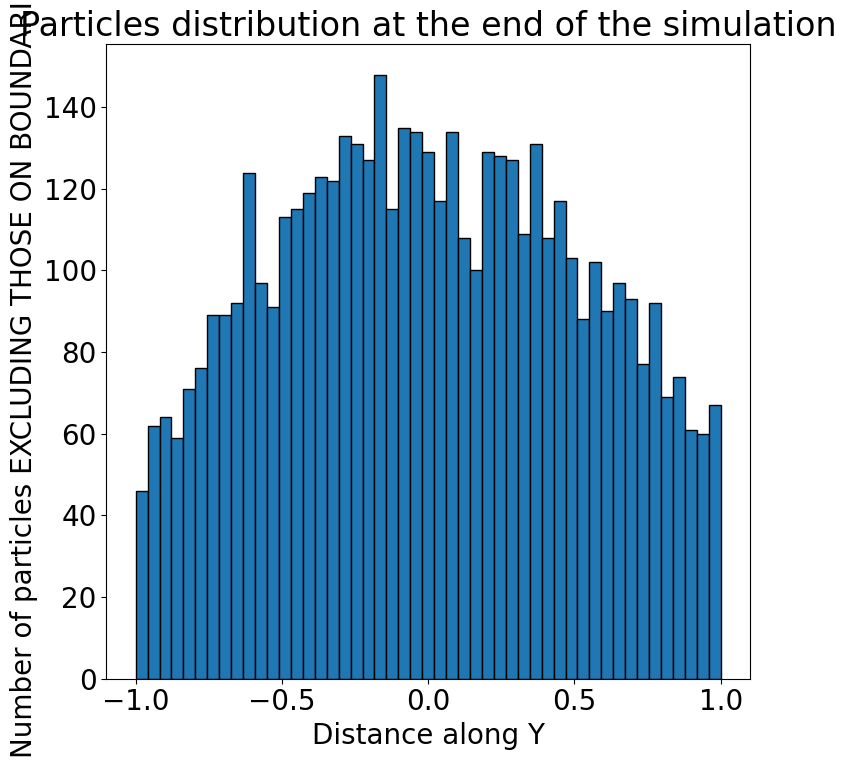
\includegraphics[width=\textwidth]{images/verticalFinalDist.png} % Replace with your image path
        \caption{Vertical distribution of particles}
        \label{fig:subplotVertFinal}
    \end{subfigure}
    \hfill
    \begin{subfigure}[b]{0.45\textwidth}
        \centering
        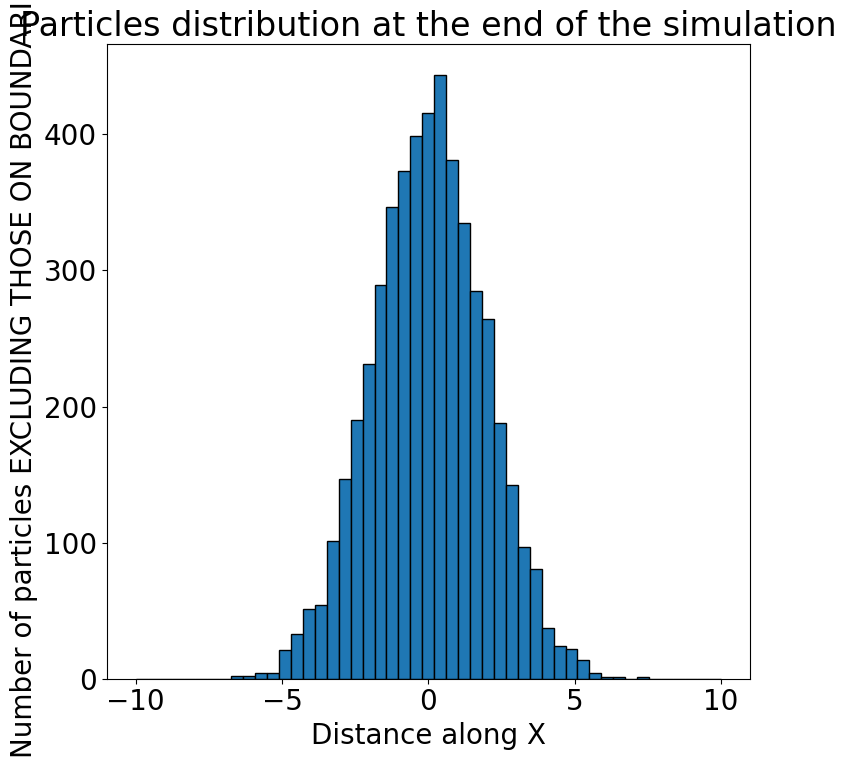
\includegraphics[width=\textwidth]{images/horizontalFinalDist.png} % Replace with your image path
        \caption{Horizontal distribution of particles}
        \label{fig:subplotHorFinal}
    \end{subfigure}
    \caption{Absorbing boundaries}
    \label{fig:Absorption}
\end{figure}

\subsection{Non-absorbed particles in time}
Figure \ref{fig:AbsorptionInTime} show the number of free particles, i.e. those that were not absorbed, throughout time. The probability for the particles to be absorbed by the boundaries of the fracture is:
\begin{equation}
    p_a = 100 \%
\end{equation}
\begin{figure}[htbp]
    \centering
    \begin{subfigure}[b]{0.45\textwidth}
        \centering
        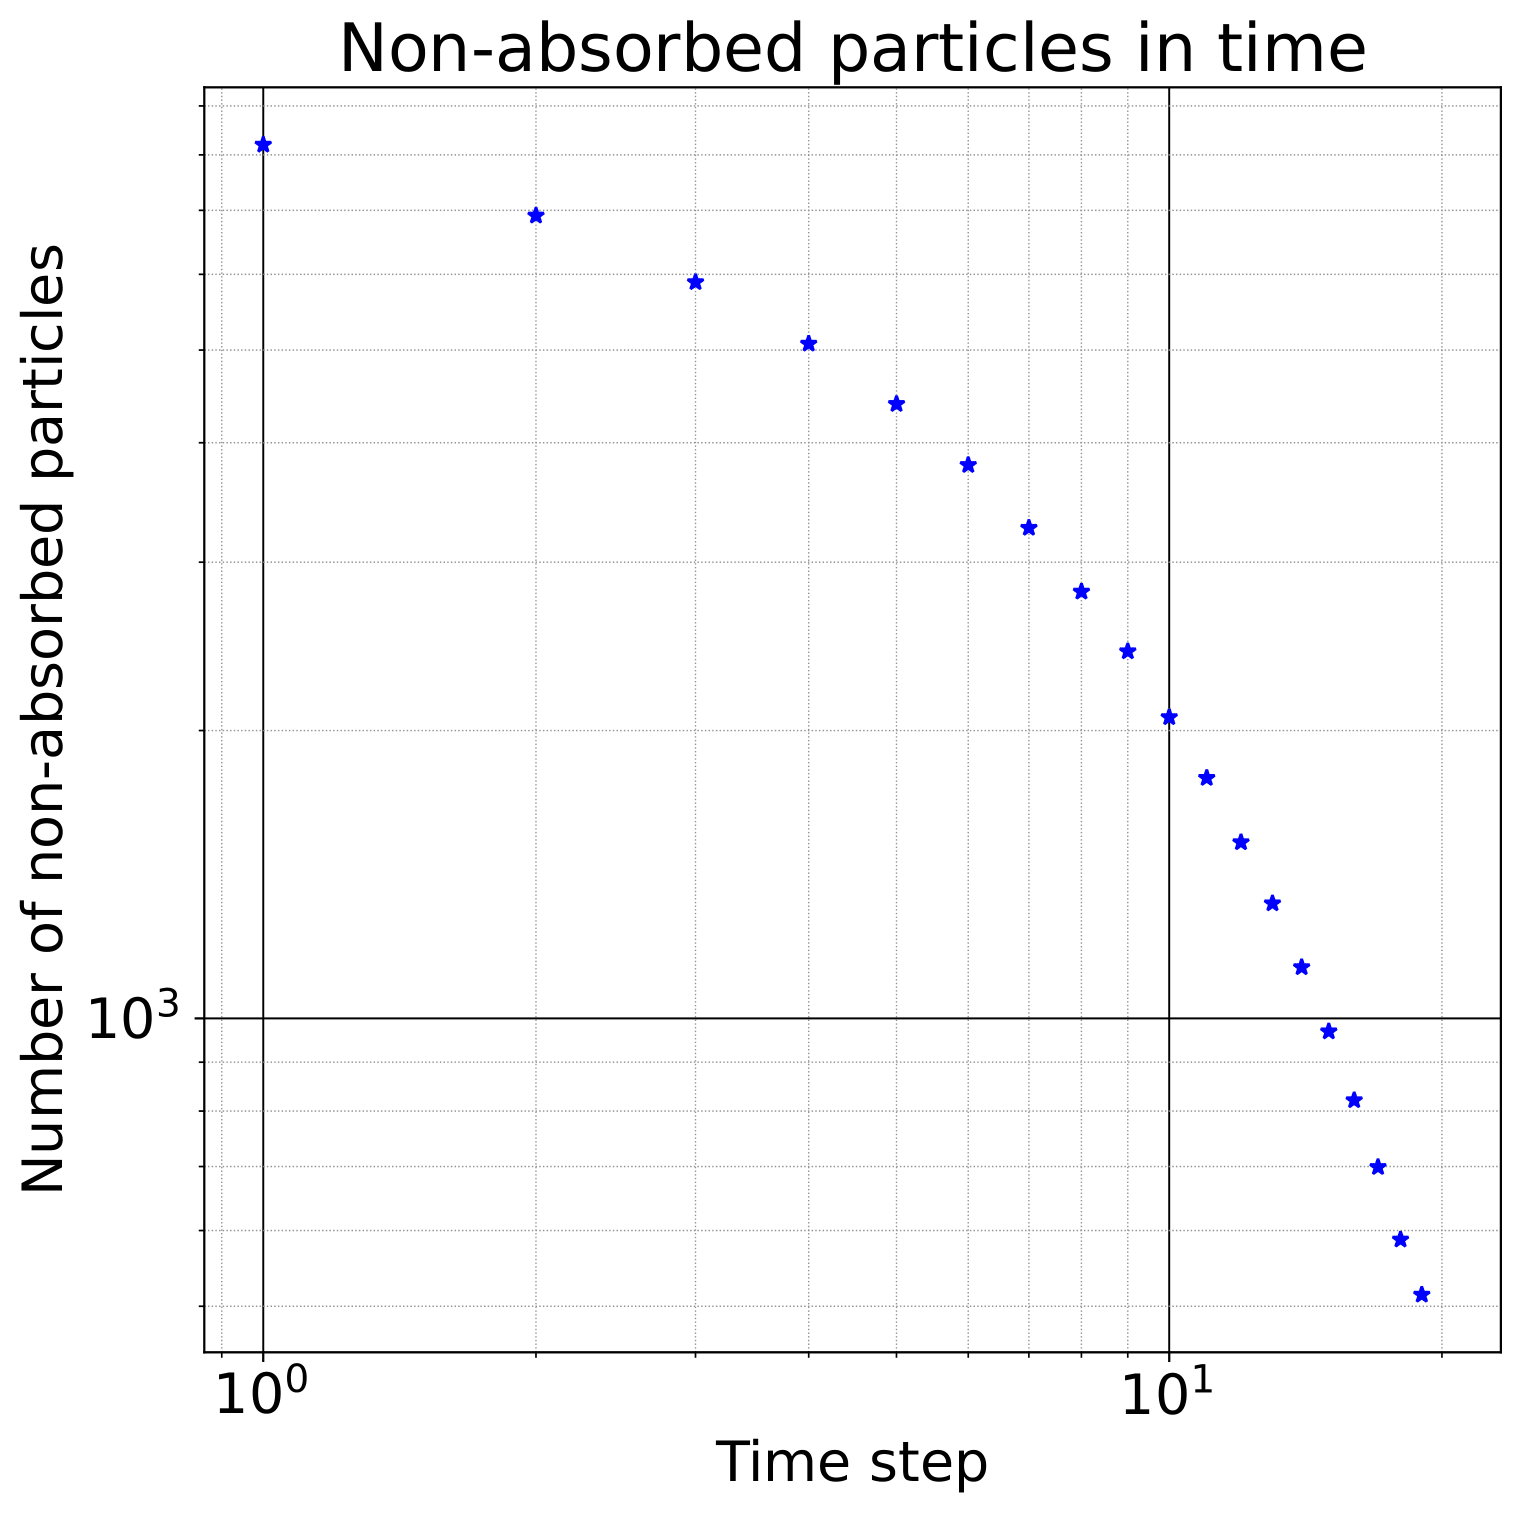
\includegraphics[width=\textwidth]{images/nonAbsParticles.png}
        \caption{Non-absorbed particles in time}
        \label{fig:subplotNonAbsPart}
    \end{subfigure}
    \hfill
    \begin{subfigure}[b]{0.45\textwidth}
        \centering
        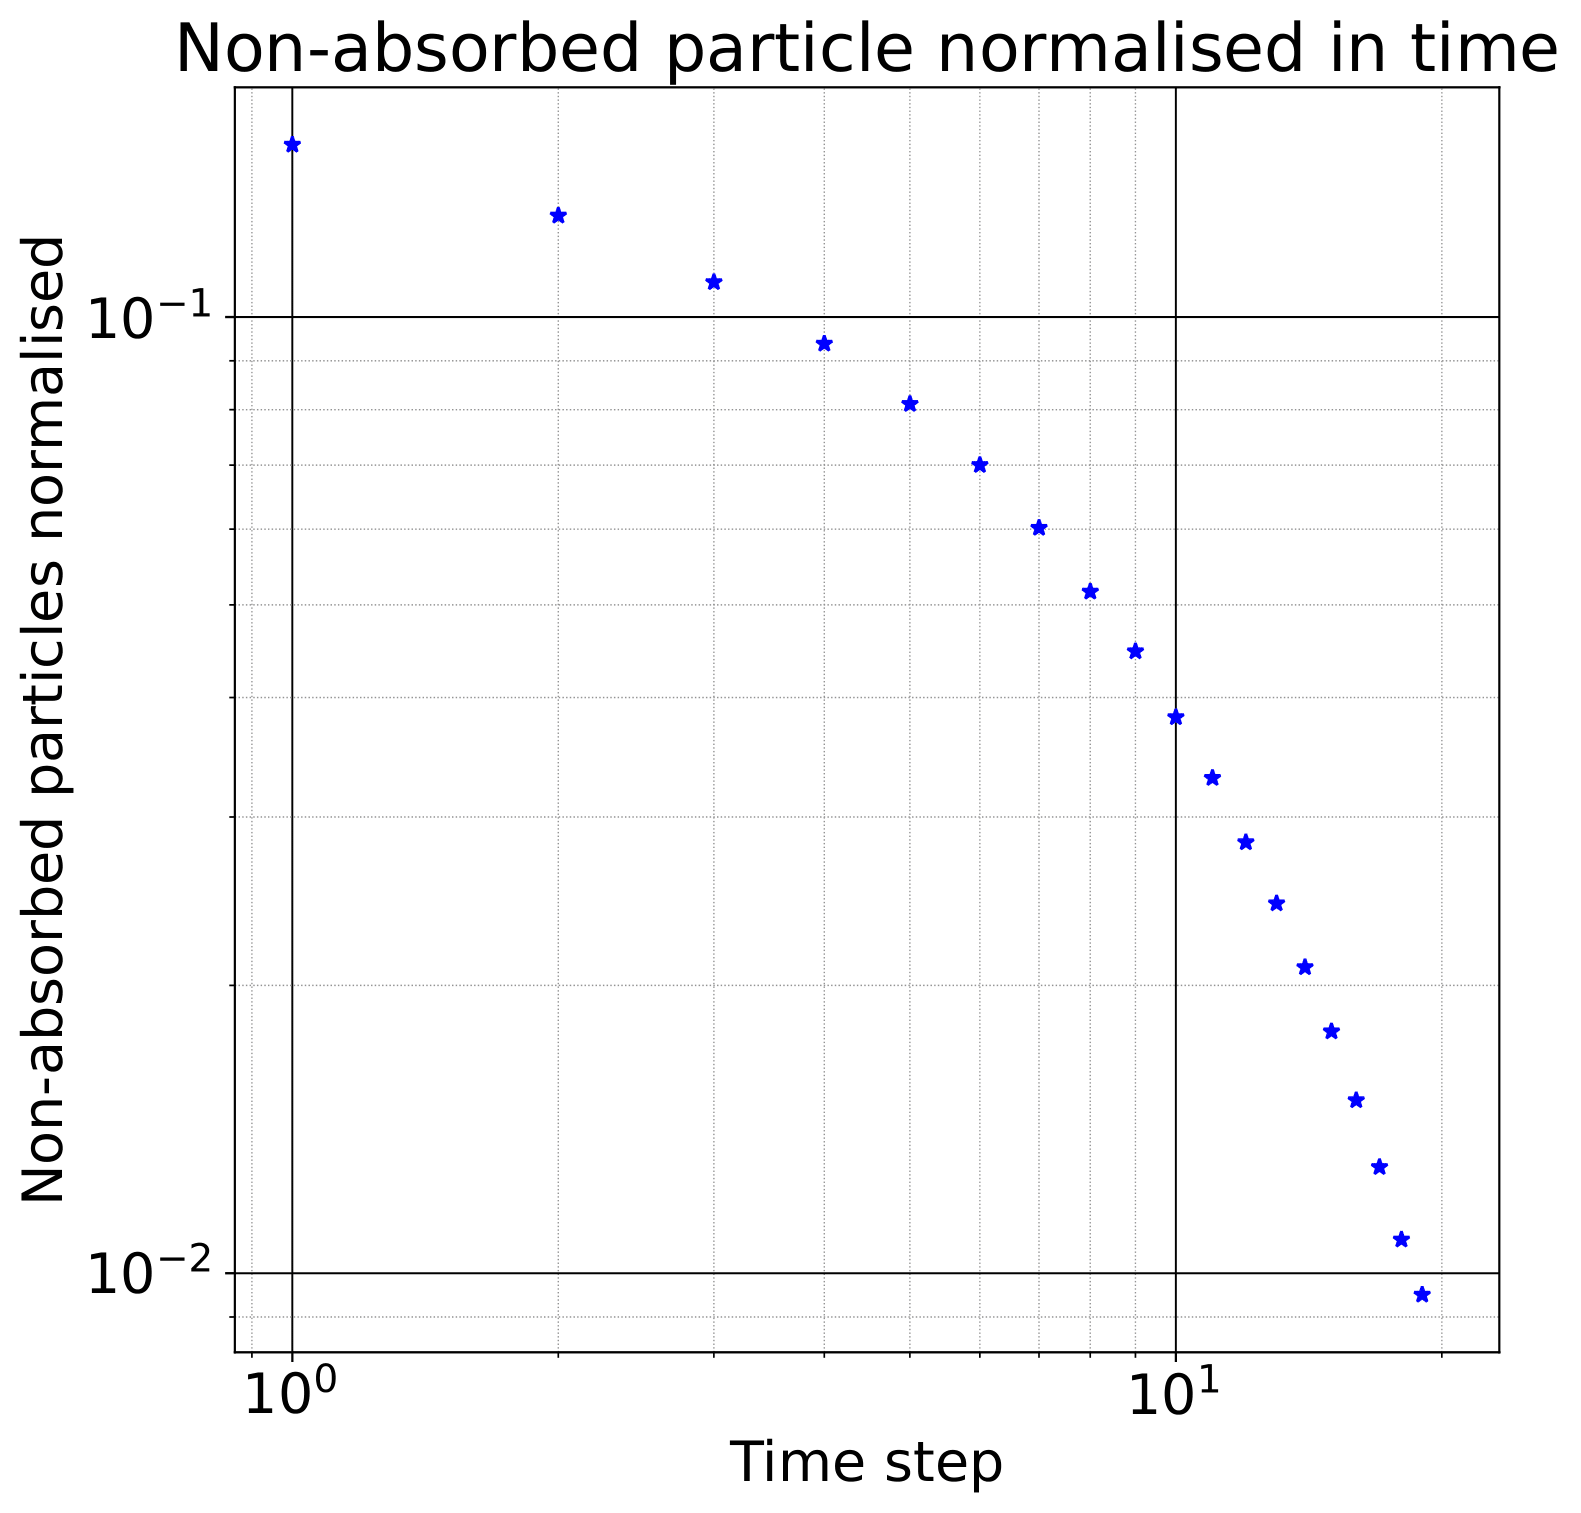
\includegraphics[width=\textwidth]{images/nonAbsParticlesNorm.png}
        \caption{Normalised number of non-absorbed particles in time}
        \label{fig:subplotNonAbsPartNorm}
    \end{subfigure}
    \caption{Non-absorbed particles in time normalised with initial total number of particles}
    \label{fig:AbsorptionInTime}
\end{figure}

\FloatBarrier  % Prevents figures from floating past this point
\section{Well-mixed vs diffusion-limited}
\subsection{Survival time distribution and reaction rates}
\begin{figure}[htbp]
    \centering
    \begin{subfigure}[b]{0.45\textwidth}
        \centering
        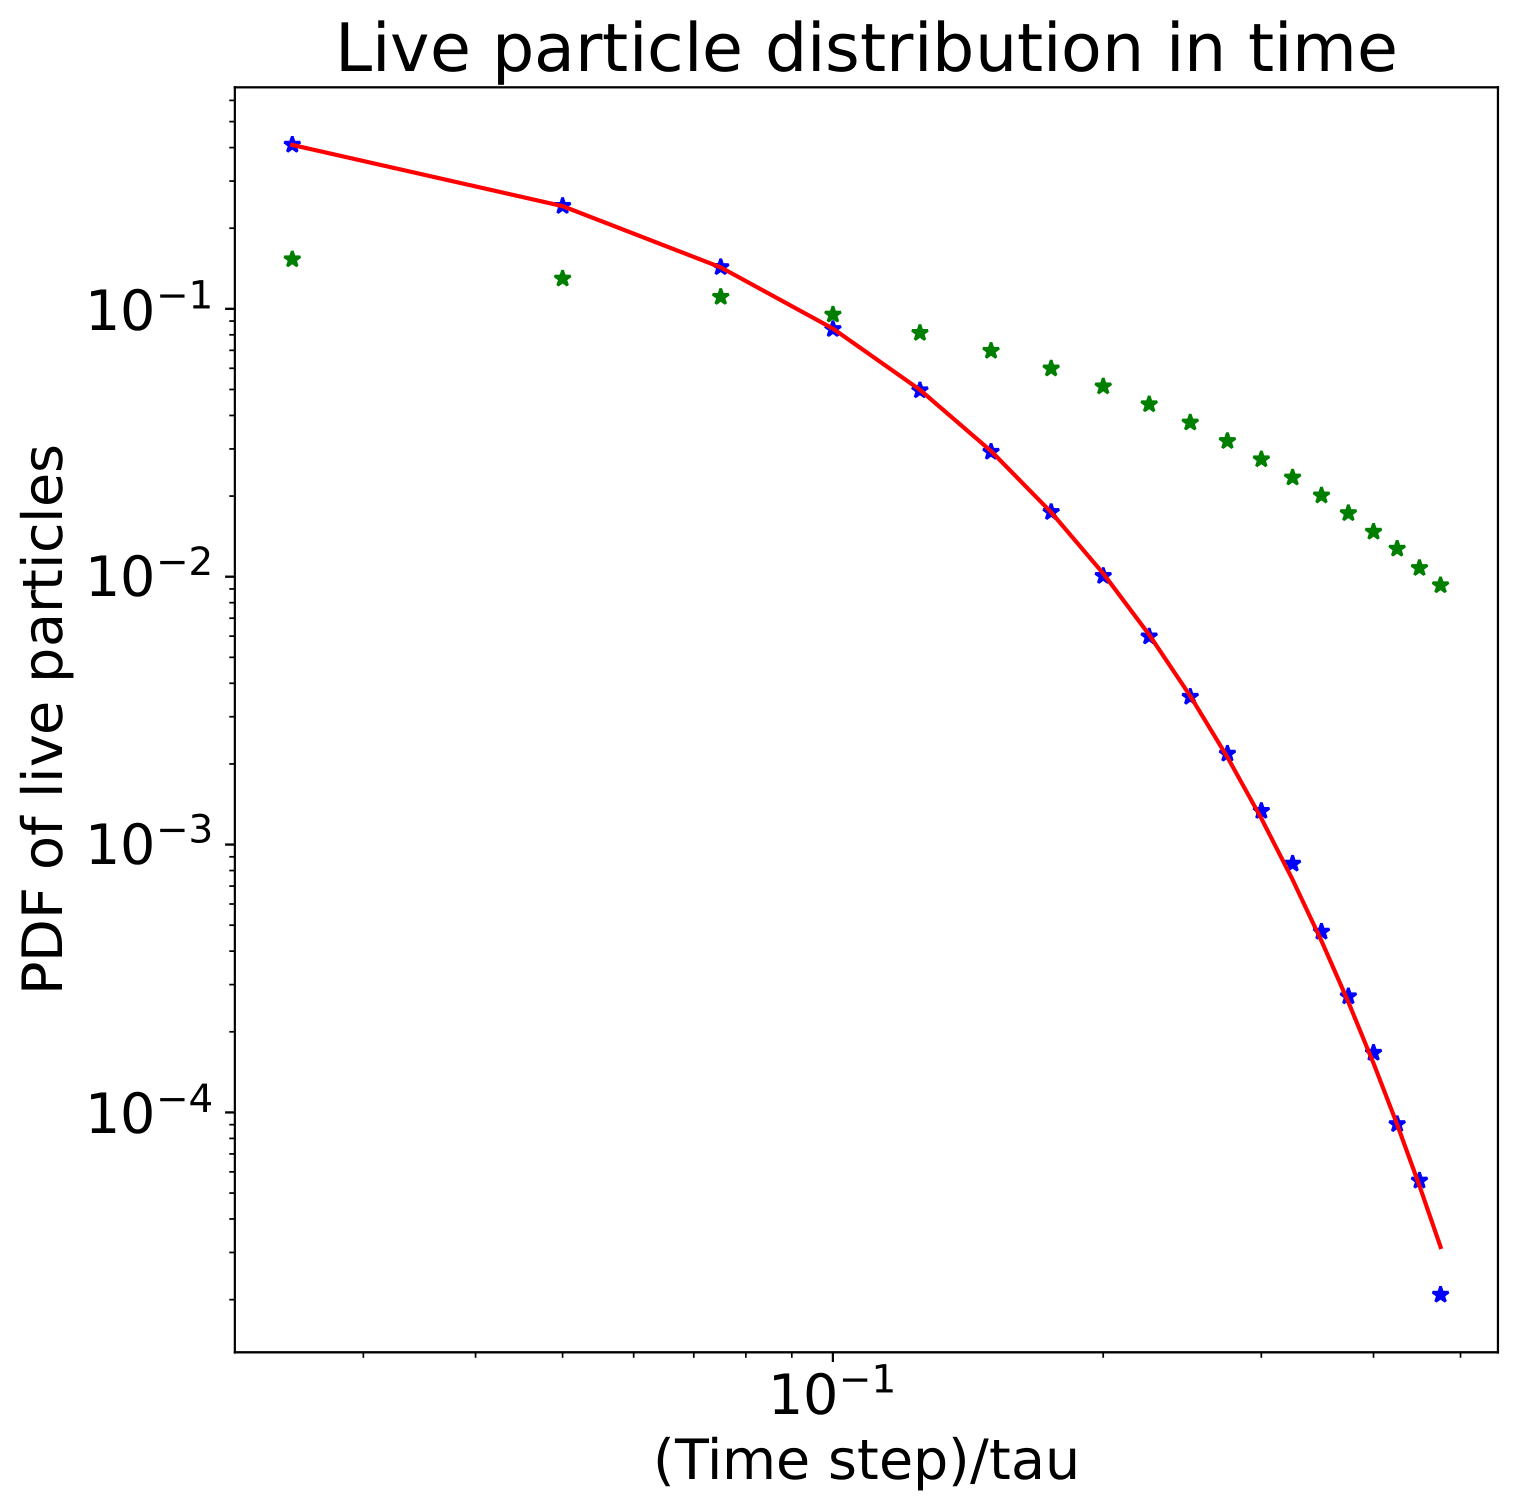
\includegraphics[width=\textwidth]{images/survTimeDistCompare.png}
        \caption{Survival time distribution curves from experimental well-mixed scenario and diffusion-limited experimental case.}
    \end{subfigure}
    \hfill
    \begin{subfigure}[b]{0.45\textwidth}
        \centering
        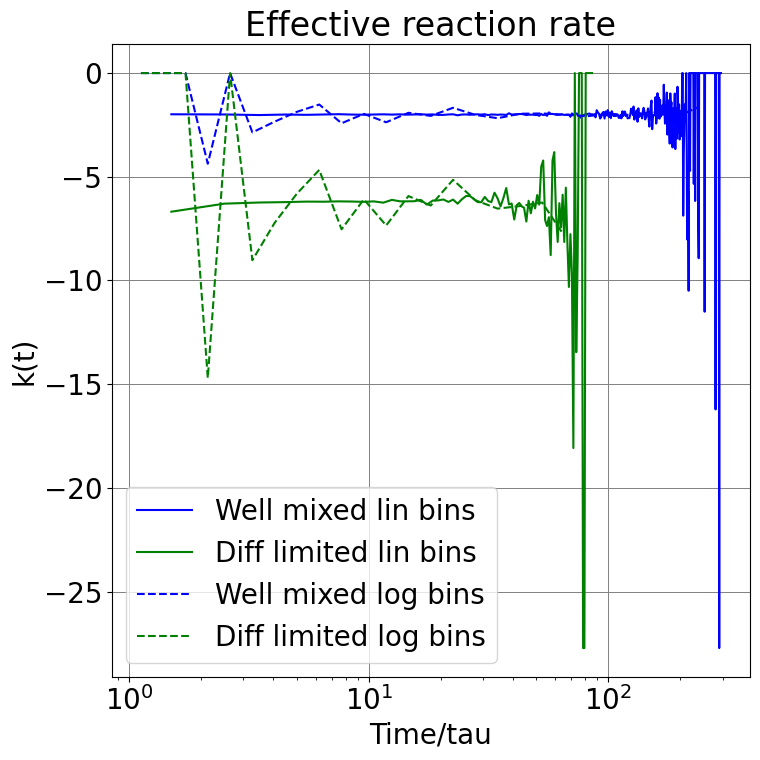
\includegraphics[width=\textwidth]{images/compareDecayDegradationRates.png}
        \caption{Reaction rates from experimental well-mixed scenario and diffusion-limited experimental case.}
    \end{subfigure}
    \caption{$10^6$ particles and 500 time steps. The value of the exponent k for the analytical case is 0.5.}
    \label{fig:survTimeAndRatesNorm}
\end{figure}

\FloatBarrier  % Prevents figures from floating past this point
\subsection{Adsorbing boundaries: survival time distributions and effective reaction rates}
\subsubsection{Effect of diffusivity coefficient}
\begin{figure}[htbp]
    \centering
    \begin{subfigure}[b]{0.45\textwidth}
        \centering
        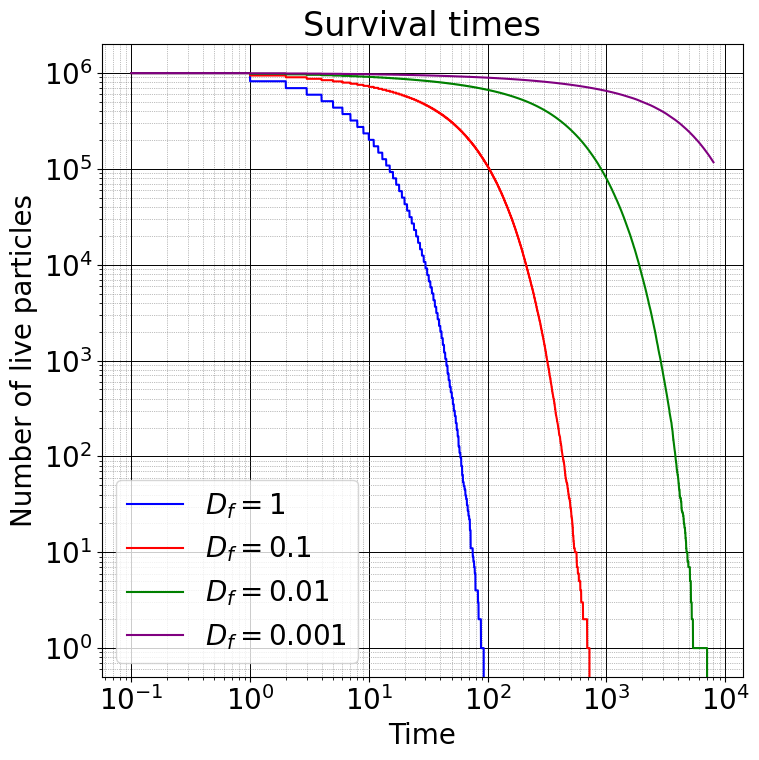
\includegraphics[width=\textwidth]{images/survTimeDistCompareDiff.png}
        \caption{Effect of diffusivity coefficient on survival time distribution for adsorbing boundary conditions}
    \end{subfigure}
    \hfill
    \begin{subfigure}[b]{0.45\textwidth}
        \centering
        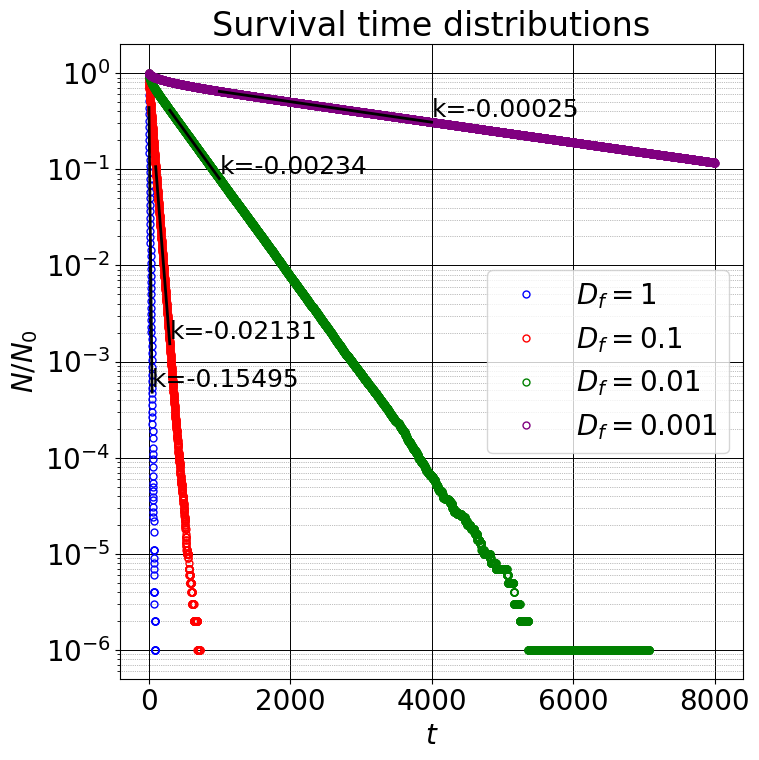
\includegraphics[width=\textwidth]{images/survTimeDistCompareDiffNorm.png}
        \caption{Effect of diffusivity coefficient on normalised survival time distribution for adsorbing boundary conditions}
    \end{subfigure}
    \caption{$10^6$ particles and 8000 time steps. The fracture's width is 2.}
    \label{fig:survTimeDiff}
\end{figure}

\begin{figure}[htbp]
    \centering
    \begin{subfigure}[b]{0.45\textwidth}
        \centering
        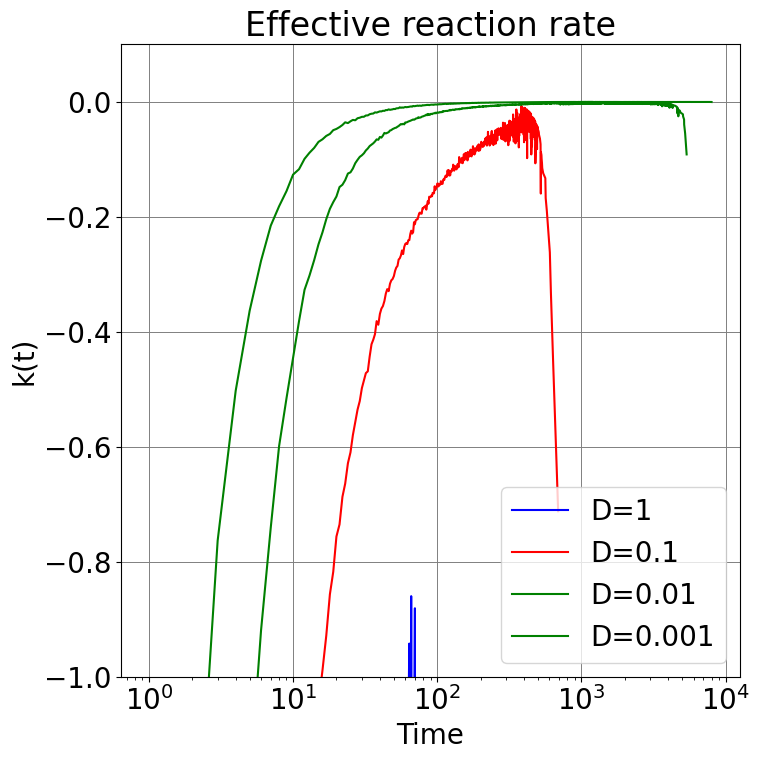
\includegraphics[width=\textwidth]{images/compareAdsRatesDiff.png}
        \caption{Reaction rates for different diffusivity values}
    \end{subfigure}
    \hfill
    \begin{subfigure}[b]{0.45\textwidth}
        \centering
        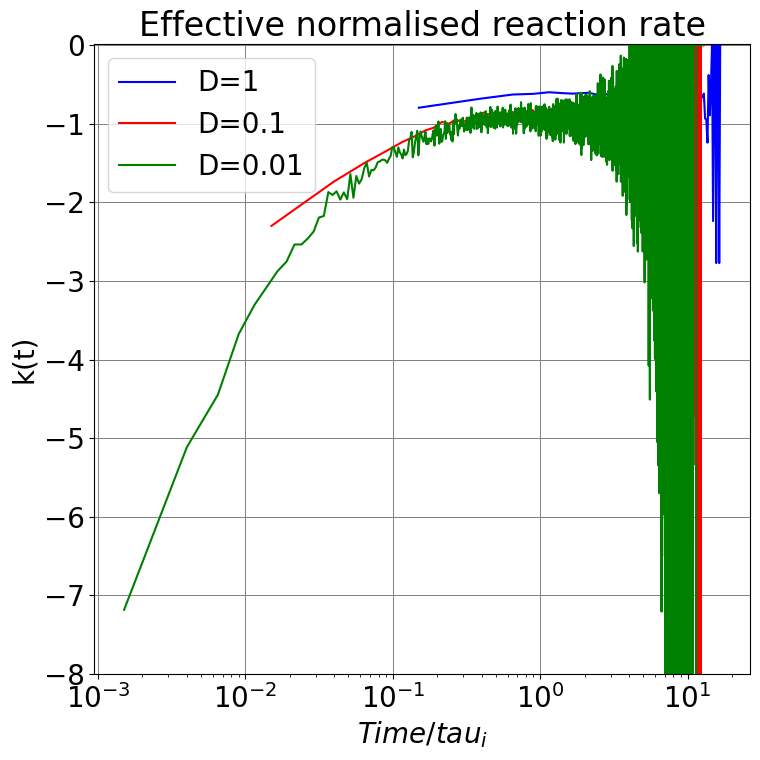
\includegraphics[width=\textwidth]{images/compareDiffNormAdsRates.png}
        \caption{Reaction rates for different diffusivity values from normalised surv time dist}
    \end{subfigure}
    \caption{Reaction rates for different diffusivity values}
    \label{fig:reactionRatesDiff}
\end{figure}

\FloatBarrier  % Prevents figures from floating past this point
\subsubsection{Effect of fracture's aperture}
\begin{figure}[htbp]
    \centering
    \begin{subfigure}[b]{0.45\textwidth}
        \centering
        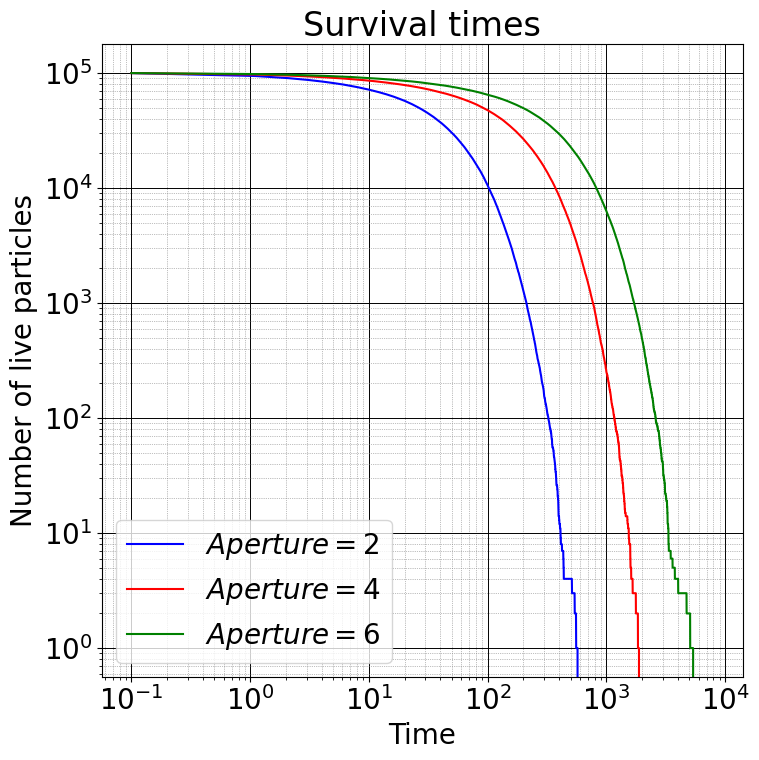
\includegraphics[width=\textwidth]{images/survTimeDistCompareApe.png}
        \caption{Effect of aperture's width on survival time distribution for adsorbing boundary conditions}
    \end{subfigure}
    \hfill
    \begin{subfigure}[b]{0.45\textwidth}
        \centering
        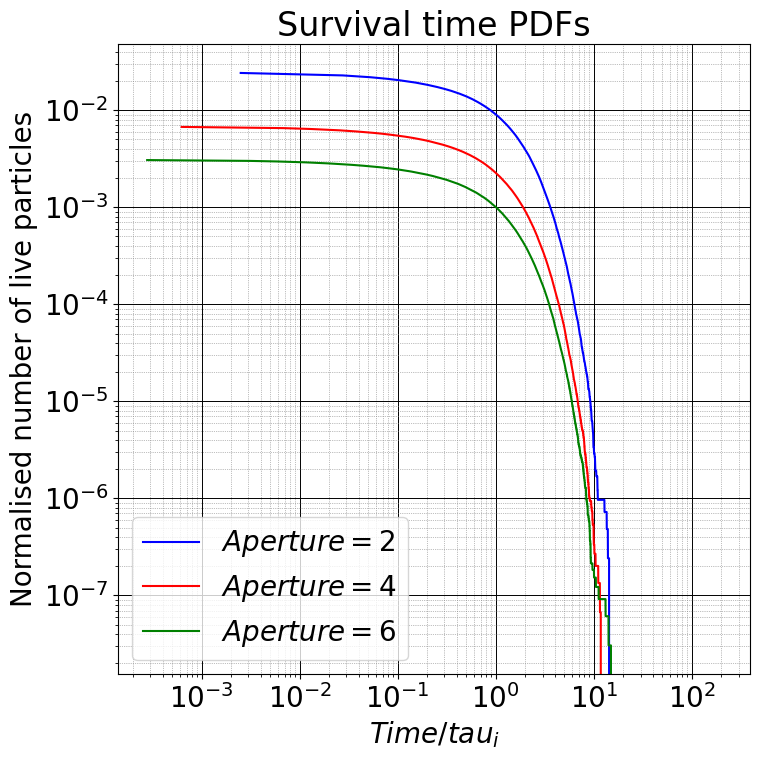
\includegraphics[width=\textwidth]{images/survTimeDistCompareApeNorm.png}
        \caption{Effect of aperture's width on normalised survival time distribution for adsorbing boundary conditions}
    \end{subfigure}
    \caption{$10^6$ particles and 8000 time steps. The diffusivity coefficient is 0.1.}
    \label{fig:survTimeape}
\end{figure}

\begin{figure}[htbp]
    \centering
    \begin{subfigure}[b]{0.45\textwidth}
        \centering
        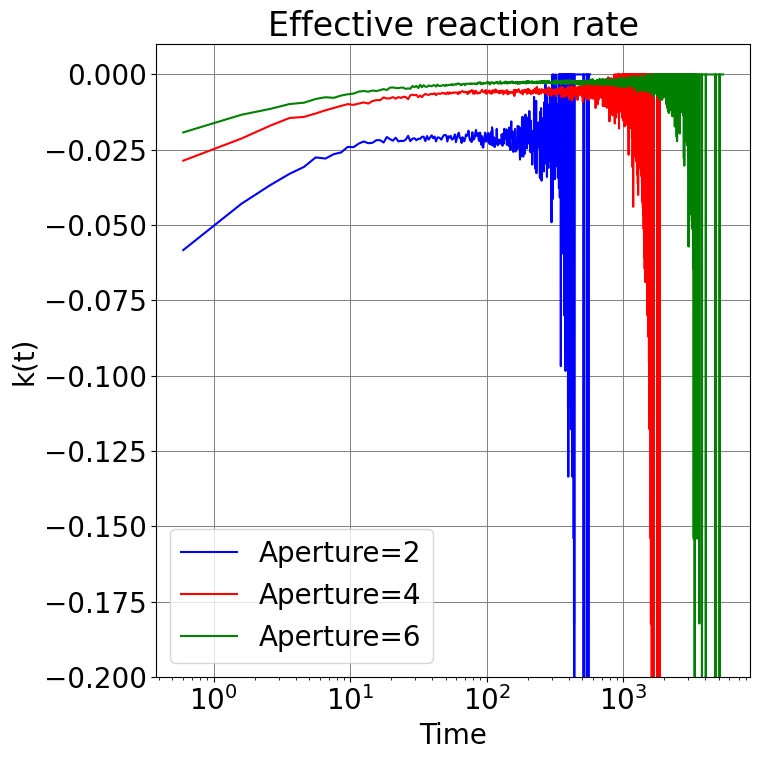
\includegraphics[width=\textwidth]{images/compareAdsRatesApe.png}
        \caption{Reaction rates for different values of apertures' width}
    \end{subfigure}
    \hfill
    \begin{subfigure}[b]{0.45\textwidth}
        \centering
        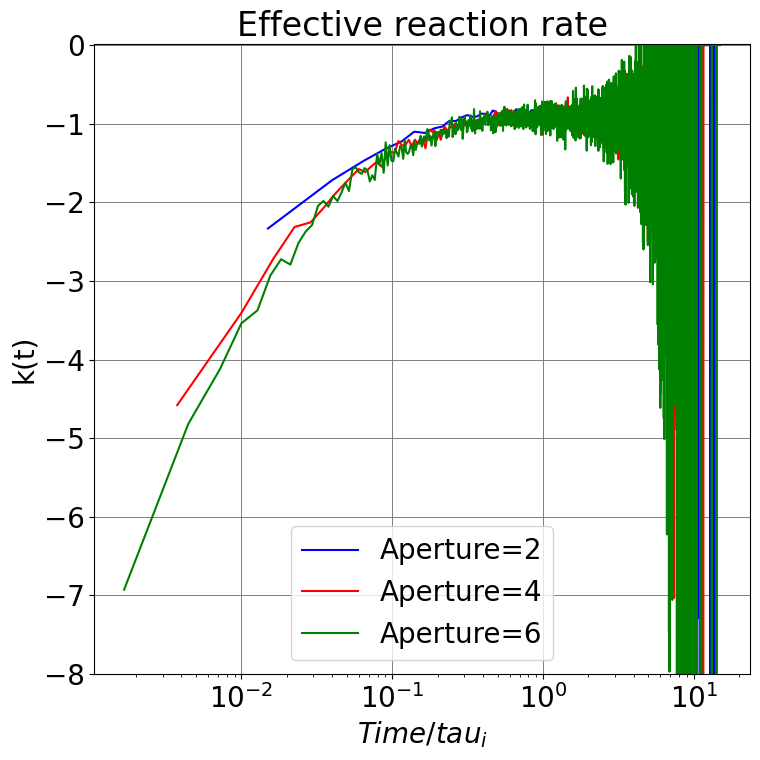
\includegraphics[width=\textwidth]{images/compareApeNormAdsRates.png}
        \caption{Reaction rates for different values of aperture's width from normalised survival time distributions}
    \end{subfigure}
    \caption{Reaction rates for different apertures' width}
    \label{fig:reactionRatesApe}
\end{figure}

\FloatBarrier  % Prevents figures from floating past this point
\section{Matrix diffusion}
For each particle crossing from the fracture to the porous matrix, a random number from a uniform distribution over the interval 0 and 1 is drawn. If this number is higher than a threshold then the particle crosses the boundary otherwise it is elastically reflected. Following the approach of \cite{salamon2006review} we set the probability of a particle crossing the fracture-porous matrix boundary equal to:
\begin{equation}
    P_f = \frac{\sqrt{D_f}}{\sqrt{D_f}+\sqrt{D_m}}
\end{equation}
\begin{figure}[htbp]
    \centering
    \begin{subfigure}[b]{0.45\textwidth}
        \centering
        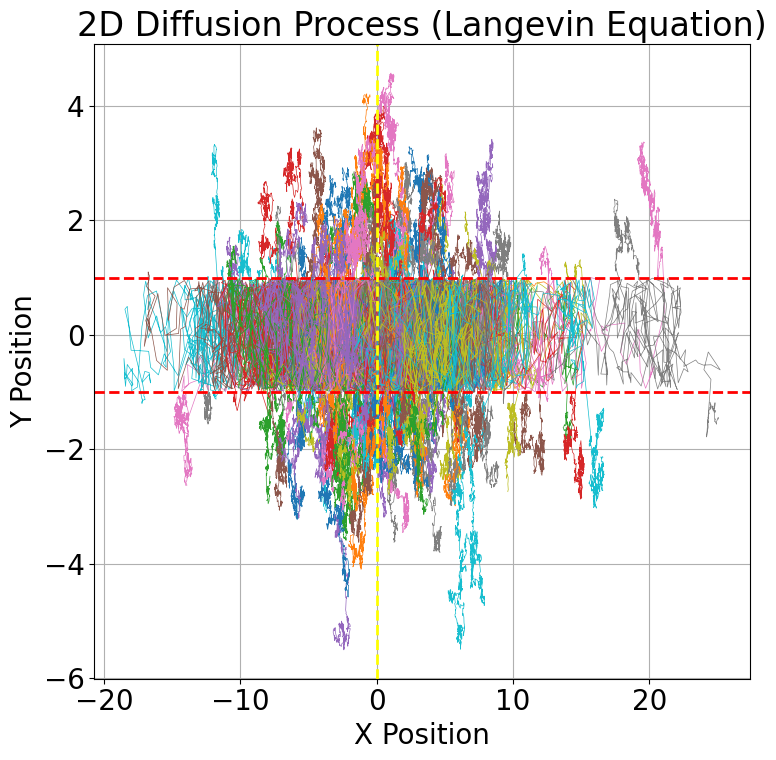
\includegraphics[width=\textwidth]{images/trajectoriesMatrixDiffusion.png}
        \caption{Trajectories from matrix diffusion implemented according to Semra 1993 and using Df=0.1 and Dm=0.001 and 100 particles and 1000 time steps}
        \label{fig:MatDiff}
    \end{subfigure}
    \hfill
    \begin{subfigure}[b]{0.45\textwidth}
        \centering
        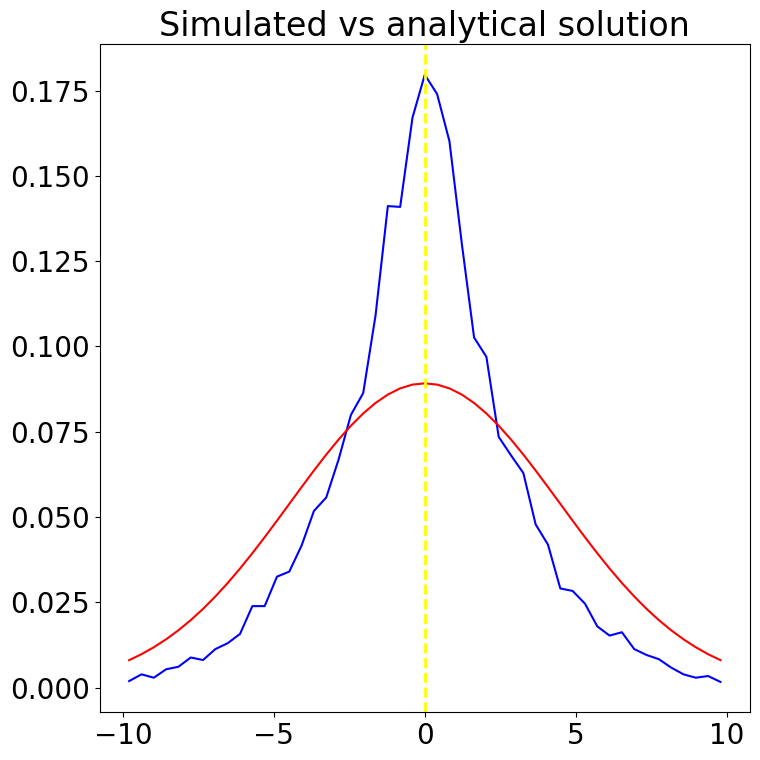
\includegraphics[width=\textwidth]{images/verificationMatrixDiffusion.png}
        \caption{Analytical solution vs numerical experiment using matrix diffusion and $10^4$ particles and $10^4$ time steps and recorded at t=100 time steps}
        \label{fig:MatrixDiffusionVerification}
    \end{subfigure}
    \caption{Verification against analytical solution for infinite domain}
    \label{fig:MatrixDiffusion}
\end{figure}
The table \ref{fig:MatrixDiffusionVerification} highlights the difference between the diffusion coefficient of the fracture and the one of the porous matrix: once a particle escapes from the fracture, its jumps are 100 times smaller compared to those that still live in the fracture. It follows that, the more impacts the more particles cross the border and the higher the concentration. Interesting enough, if the probability of matrix-to-fracture crossing is zero, after $10^4$ time steps no particles is left in the fracture, as shown in Figure \ref{fig:finalPosMatrixDiff}.
\begin{figure}[h]
    \centering
    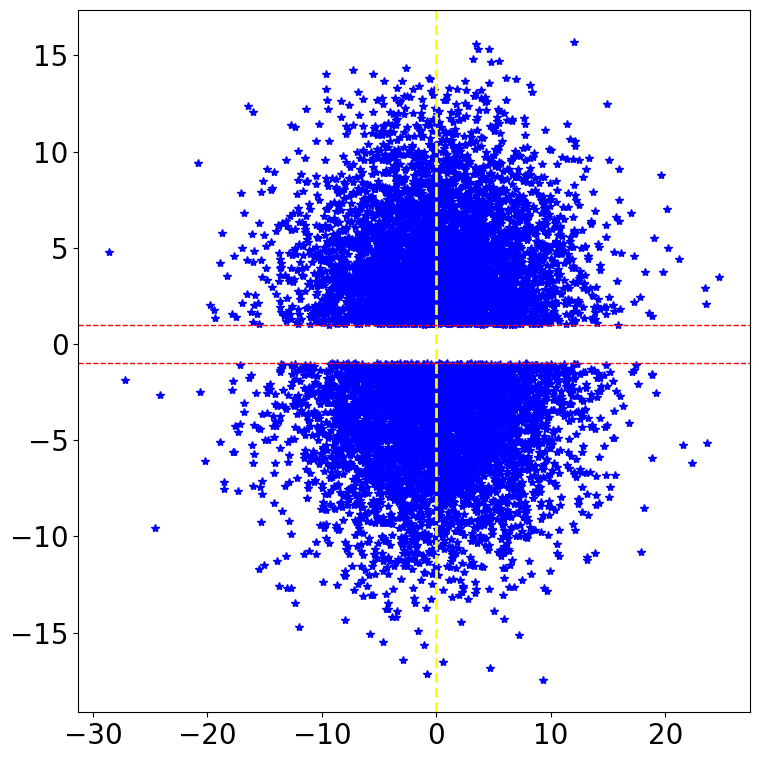
\includegraphics[width=0.5\textwidth]{images/finalPositionsMatrixDiffusion.png}
    \caption{Final position of $10^4$ particles after $10^4$ time steps}
    \label{fig:finalPosMatrixDiff}
\end{figure}

\FloatBarrier  % Prevents figures from floating past this point
\subsection{Verification: no probabilistic crossing between different diffusivity}
\begin{figure}[htbp]
    \centering
    \begin{subfigure}[b]{0.45\textwidth}
        \centering
        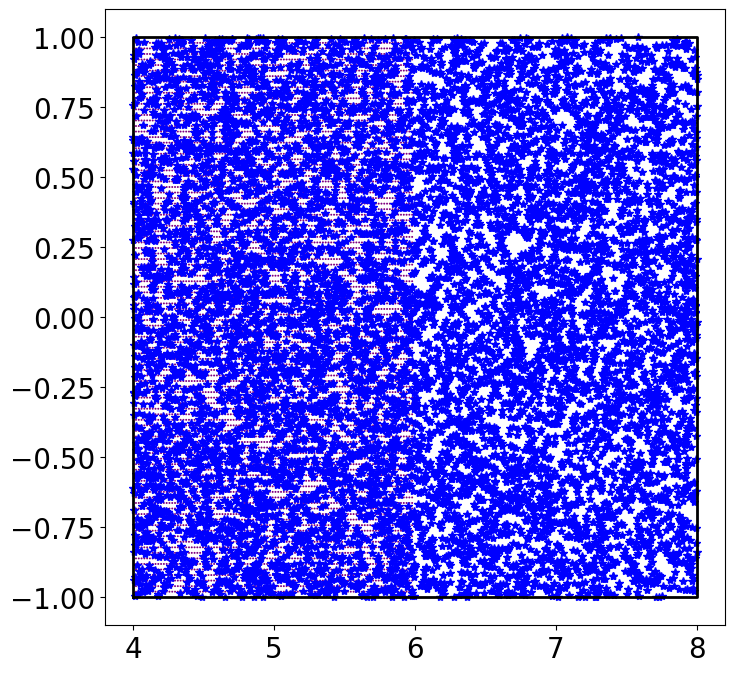
\includegraphics[width=\textwidth]{images/positionsDl01Dr01Rl0Rr0.png}
        \caption{No probability condition on crossing between the two diffusivity regions and Dl = Dr = 0.1}
    \end{subfigure}
    \hfill
    \begin{subfigure}[b]{0.45\textwidth}
        \centering
        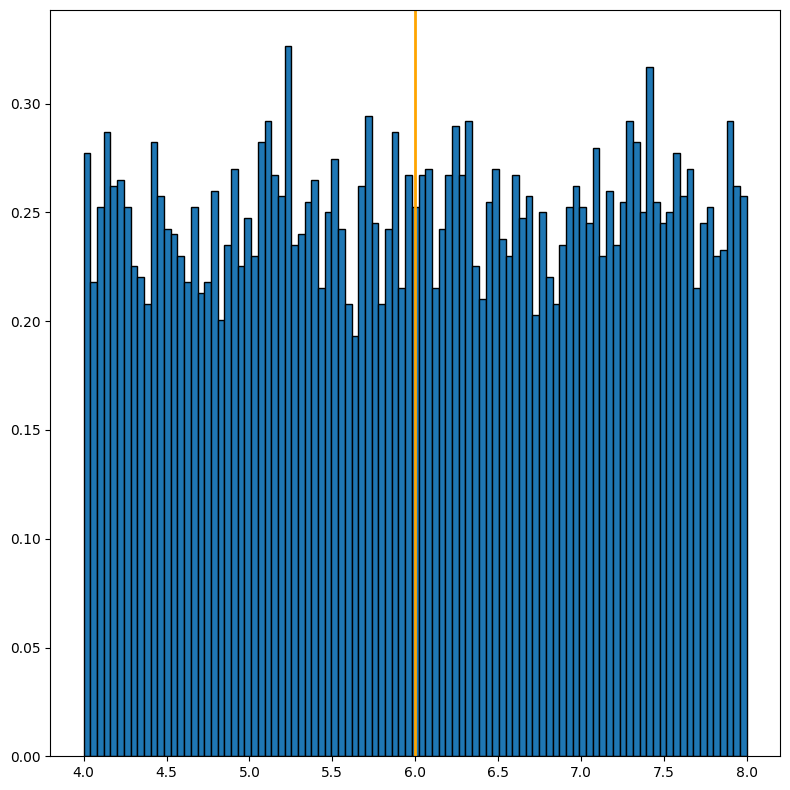
\includegraphics[width=\textwidth]{images/histDl01Dr01Rl0Rr0.png}
        \caption{Normalised histogram of particles' distribution along X at the end of the simulation}
    \end{subfigure}
    \caption{1e4 particles, 1e4 time steps, dt=1}
    \label{fig:MatrixDiffusion1}
\end{figure}

\begin{figure}[htbp]
    \centering
    \begin{subfigure}[b]{0.45\textwidth}
        \centering
        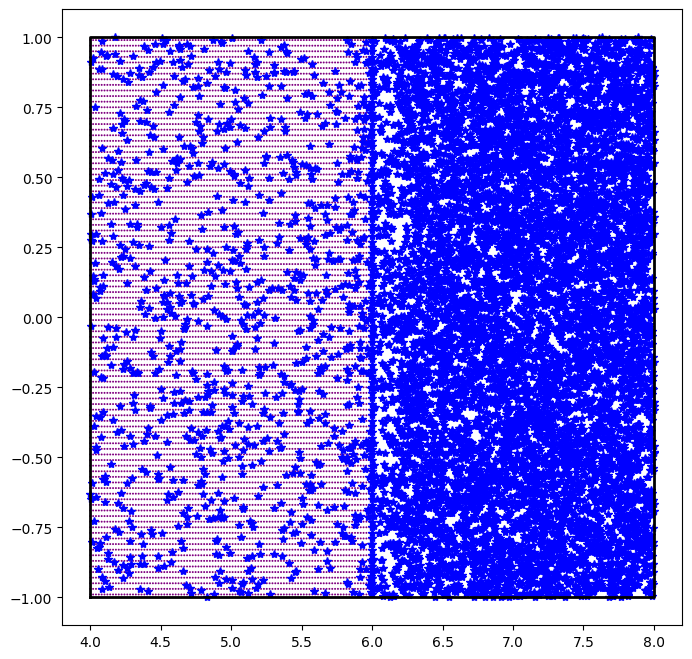
\includegraphics[width=\textwidth]{images/positionsDl01Dr001Rl0Rr0.png}
        \caption{No probability condition on crossing between the two diffusivity regions and Dl = 0.1 while Dr = 0.01}
    \end{subfigure}
    \hfill
    \begin{subfigure}[b]{0.45\textwidth}
        \centering
        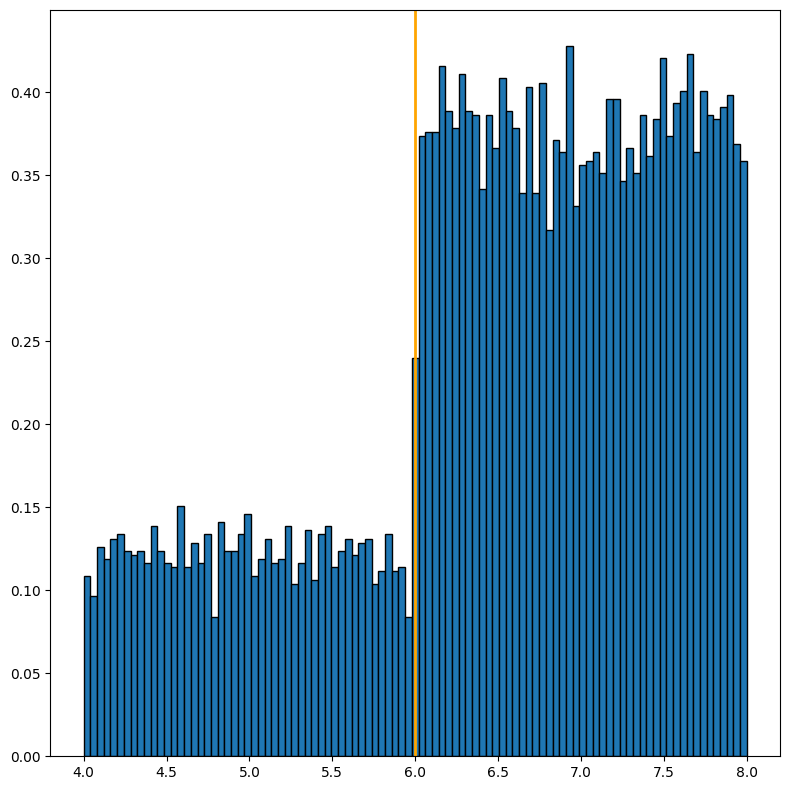
\includegraphics[width=\textwidth]{images/histDl01Dr001Rl0Rr0.png}
        \caption{Normalised histogram of particles' distribution along X at the end of the simulation}
    \end{subfigure}
    \caption{1e4 particles, 1e4 time steps, dt=1}
    \label{fig:MatrixDiffusion2}
\end{figure}

\FloatBarrier  % Prevents figures from floating past this point
\subsection{Verification: probabilistic boundary between different diffusivity}
\begin{figure}[htbp]
    \centering
    \begin{subfigure}[b]{0.45\textwidth}
        \centering
        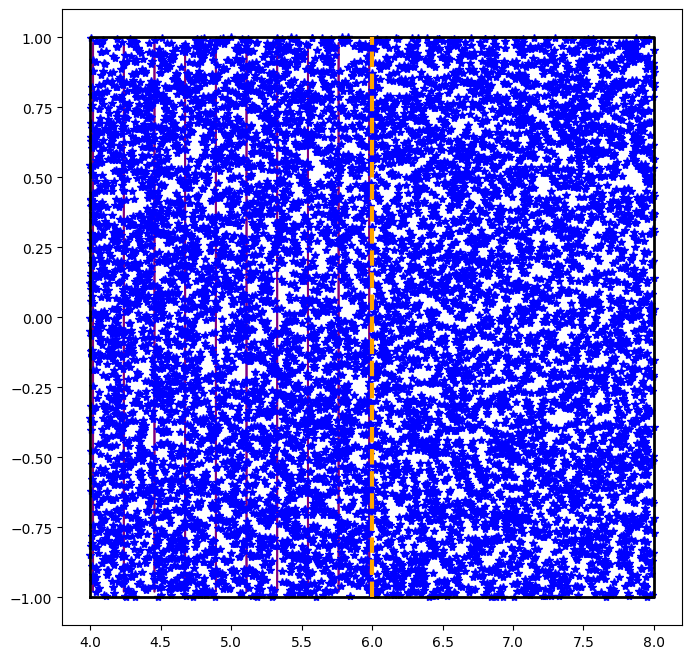
\includegraphics[width=\textwidth]{images/positionsDl01Dr01RlPlRrPr.png}
        \caption{Probability condition on crossing between the two diffusivity regions and Dl = Dr = 0.1}
    \end{subfigure}
    \hfill
    \begin{subfigure}[b]{0.45\textwidth}
        \centering
        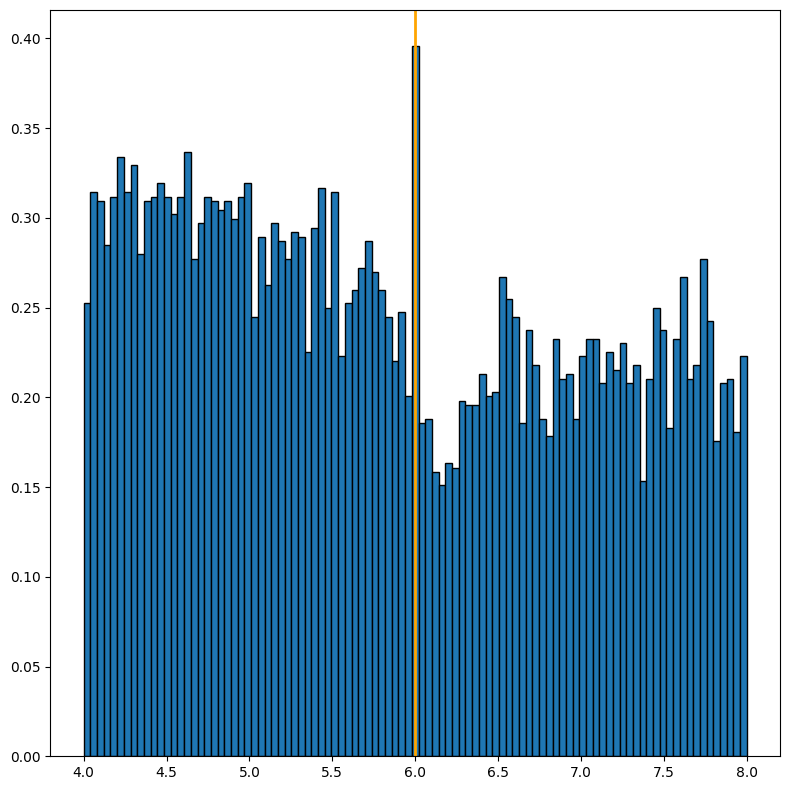
\includegraphics[width=\textwidth]{images/histDl01Dr01RlPlRrPr.png}
        \caption{Normalised histogram of particles' distribution along X at the end of the simulation}
    \end{subfigure}
    \caption{1e4 particles, 1e4 time steps, dt=1}
    \label{fig:MatrixDiffusion3}
\end{figure}

\begin{figure}[htbp]
    \centering
    \begin{subfigure}[b]{0.45\textwidth}
        \centering
        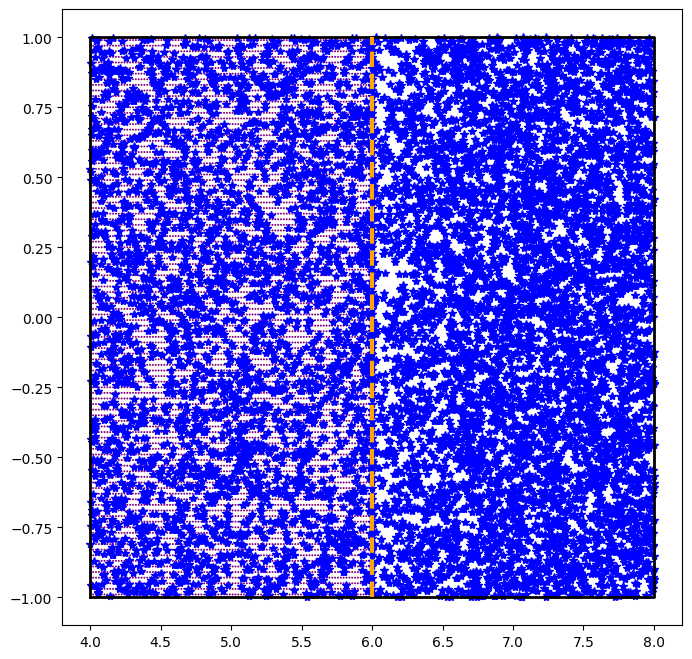
\includegraphics[width=\textwidth]{images/positionsDl01Dr001RlPlRrPr.png}
        \caption{Probability condition on crossing between the two diffusivity regions and Dl = 0.1 while Dr = 0.01}
    \end{subfigure}
    \hfill
    \begin{subfigure}[b]{0.45\textwidth}
        \centering
        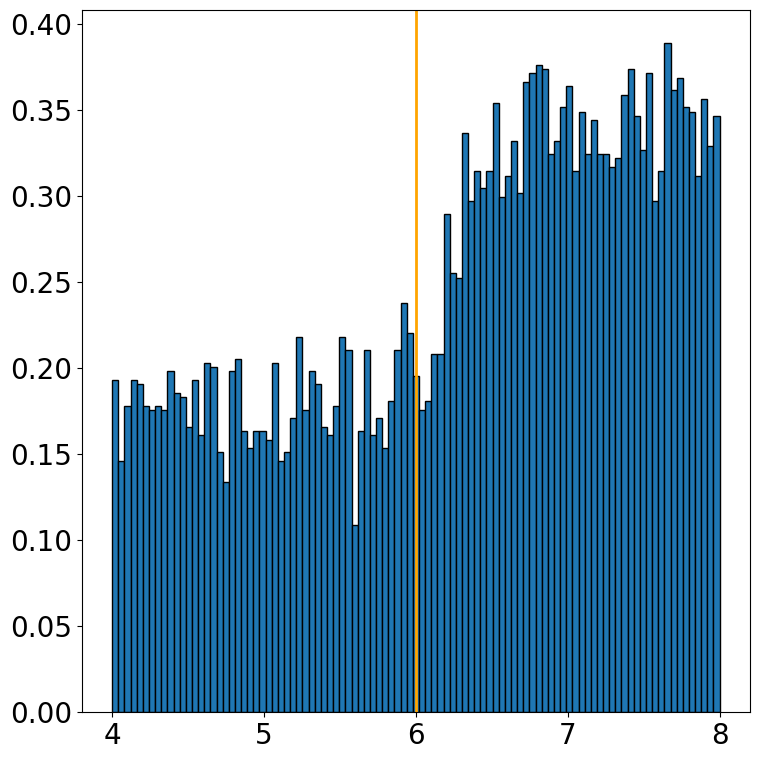
\includegraphics[width=\textwidth]{images/histDl01Dr001RlPlRrPr.png}
        \caption{Normalised histogram of particles' distribution along X at the end of the simulation}
    \end{subfigure}
    \caption{1e4 particles, 1e4 time steps, dt=1}
    \label{fig:MatrixDiffusion4}
\end{figure}

\begin{figure}[htbp]
    \centering
    \begin{subfigure}[b]{0.45\textwidth}
        \centering
        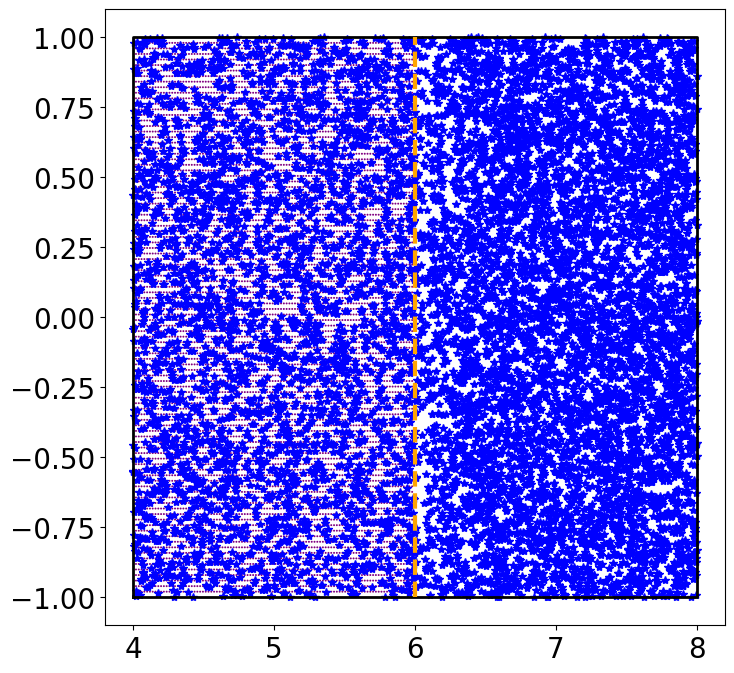
\includegraphics[width=\textwidth]{images/positionsDl01Dr001RlPlRrPr1e5ts.png}
        \caption{Probability condition on crossing between the two diffusivity regions and Dl = 0.1 while Dr = 0.01}
    \end{subfigure}
    \hfill
    \begin{subfigure}[b]{0.45\textwidth}
        \centering
        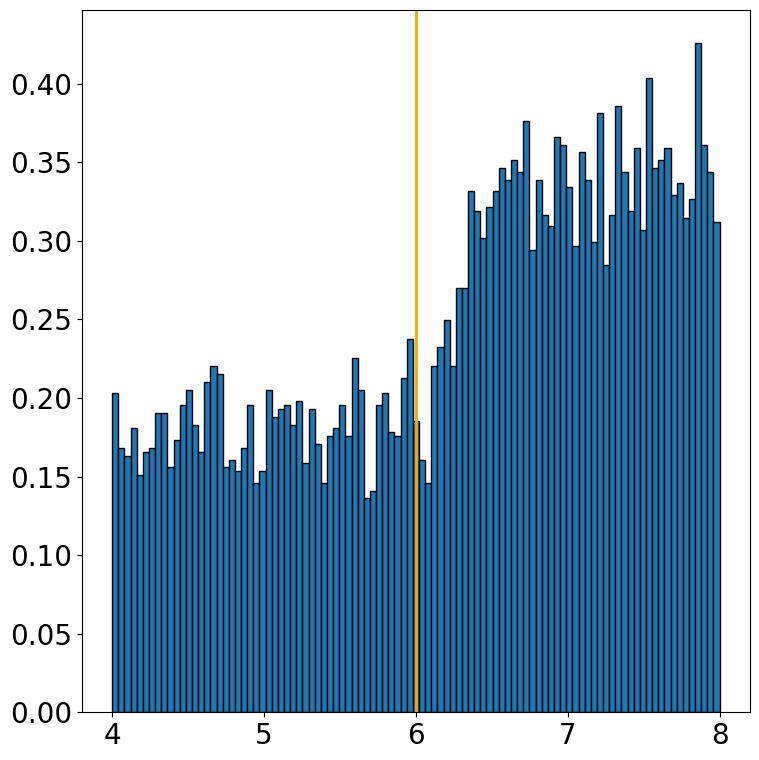
\includegraphics[width=\textwidth]{images/histDl01Dr001RlPlRrPr1e5ts.png}
        \caption{Normalised histogram of particles' distribution along X at the end of the simulation}
    \end{subfigure}
    \caption{1e4 particles, $10^5$ time steps, dt=1}
    \label{fig:MatrixDiffusion4_1e5ts}
\end{figure}


\FloatBarrier  % Prevents figures from floating past this point
\bibliographystyle{plain}  % The style of your bibliography (e.g., plain, ieee, acm, etc.)
\bibliography{references}  % Name of the .bib file without the extension

\end{document}